%
% Spektrale Modelle.tex -- Beispiel-File für teil2 
%
% (c) 2023 Dmitry Grigoriev, OST Ostschweizer Fachhochschule
%
% !TEX root = ../../buch.tex
% !TEX encoding = UTF-8
%
\section{Meteorologische Modelle in der Wettervorhersage
\label{spektral:section:modelle}}
\rhead{Meteorologische Modelle}
\begin{figure}
	\centering
	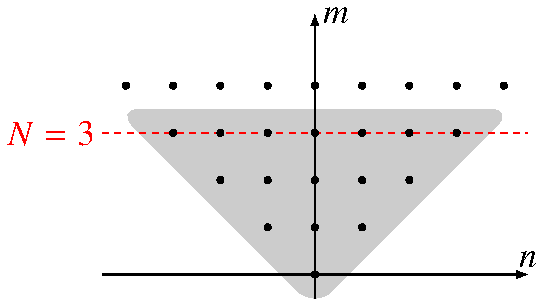
\includegraphics[height=140pt]{papers/spektral/images/triangle_truncation.pdf}
	\caption{Dreieickabschneidung}
    \label{spektral:fig:triangletrunc}
\end{figure}

Im Oktober 1973 wurde das Europäische Zentrum für mittelfristige Wettervorhersage (EZMW) gegründet \cite{spektral:ezmw} und hat die erste Vorhersagen am 1. August 1979 publiziert.
\index{EZMW}%
\index{ECMWF}%
Seit 1979 sind die Wetterprognosen, dank der spektralen Modelle, viel besser geworden.

Heute haben wir fast unendliche Rechenleistung zur Verfügung (z.~B.~Cloud-Computing), aber wir müssen trotzdem unsere Reihe \eqref{spektral:equation21} an eine fixe Anzahl der Wellen $(N)$ begrenzen.
\index{Cloud-Computing}%
In der echten Welt wird die Gleichung \eqref{spektral:equation21} so aussehen:
\begin{equation}
u(\phi, \theta, t) = \sum_{m=0}^{N}\sum_{n=-m}^{m}a_n^m(0)e^{i\sqrt{l(l+1)}t}Y_n^m(\phi, \theta).
\label{spektral:equation22}
\end{equation}
$N$ wird Modellauflösung genannt \cite[Seite 223]{spektral:NumericalWeatherPrediction} und \eqref{spektral:equation21} als {\em Dreieickabschneidung} (triangular truncation) genannt.
\index{Dreieckabschneidung}%
\index{triangular truncation}%
Wenn
z.~B.~das Model $N = 512$ hat, dann wird das Model T512 bezeichnet. 
Im Frühjahr 2006 wurden die Modelle aktualisiert. Das determinischte Model heißt jetzt T799 (vorher T511) \cite[Seite 222]{spektral:NumericalWeatherPrediction}.

Abschließend lässt sich festhalten, dass die Anwendung spektraler Modelle in der Meteorologie einen bedeutenden Fortschritt in der Erforschung und Vorhersage atmosphärischer Phänomene darstellt.
Diese Modelle ermöglichen es, komplexe Prozesse in der Atmosphäre auf einer spektralen Ebene zu analysieren und somit tiefgreifendes Verständnis zu erlangen.
Die Nutzung von spektralen Modellen hat maßgeblich zur Verbesserung der Genauigkeit von Wettervorhersagen beigetragen und ermöglicht gleichzeitig Einblicke in langfristige Klimatrends.
Doch trotz dieser Fortschritte stehen auch weiterhin Herausforderungen wie die Feinabstimmung der Modelle und die Berücksichtigung aller relevanten Faktoren.
Während wir uns in eine Ära fortschrittlicher Technologien begeben, werden spektrale Modelle zweifellos weiterhin eine Schlüsselrolle bei der Entschlüsselung der Geheimnisse unseres Wetters und Klimas spielen.
